\documentclass[mathserif, handout]{beamer}
% ======================================================================
% General LaTeX Setup for Beamer (Reusable Preamble)
% Author: Chandra Gummaluru
% ======================================================================

\documentclass[mathserif, handout]{beamer}
\setbeamertemplate{frametitle}{}

% ------------------------------------------------------------
% basic packages
% ------------------------------------------------------------
\usepackage{url}
\usepackage{ifthen}
\usepackage{enumerate}
\usepackage[font=small]{caption}
\usepackage{subcaption}
\usepackage{moresize}
\usepackage[outline]{contour}
\usepackage{transparent}
\usepackage{worldflags}
\usepackage{bm}
\usepackage{graphbox}
\usepackage{mathtools}
\usepackage{multirow}
\usepackage{fontawesome5}
\usepackage{pifont}
\usepackage{array}
\usepackage{comment}

% ------------------------------------------------------------
% math
% ------------------------------------------------------------
\DeclarePairedDelimiter{\floor}{\lfloor}{\rfloor}
\DeclarePairedDelimiter{\ceil}{\lceil}{\rceil}

% ------------------------------------------------------------
% colors
% ------------------------------------------------------------
\definecolor{hl}{RGB}{248,196,69}
\definecolor{myred}{HTML}{ED5565}
\definecolor{myorange}{HTML}{FC6E51}
\definecolor{myyellow}{HTML}{FFCE54}
\definecolor{mycyan}{HTML}{4FC1E9}
\definecolor{myblue}{HTML}{5D9CEC}

\newcommand{\graytext}[1]{\footnotesize\color{gray}#1\normalsize\color{black}}

% ------------------------------------------------------------
% symbols
% ------------------------------------------------------------
\newcommand{\cmark}{\ding{51}}
\newcommand{\xmark}{\ding{55}}

% ------------------------------------------------------------
% highlighting
% ------------------------------------------------------------
\newcommand{\reducedstrut}{\vrule width 0pt height .9\ht\strutbox depth .9\dp\strutbox\relax}
\newcommand{\highlight}[1]{%
  \begingroup\setlength{\fboxsep}{0pt}\colorbox{hl}{\reducedstrut$\displaystyle #1$\/}\endgroup}
\newcommand{\highlightc}[2]{%
  \begingroup\setlength{\fboxsep}{0pt}\colorbox{#1}{\reducedstrut$\displaystyle #2$\/}\endgroup}

% ------------------------------------------------------------
% environments (boxes)
% ------------------------------------------------------------
\usepackage{tcolorbox}
\tcbuselibrary{skins}

\newtcolorbox{thmbox}[1][]{colback=gray!30!white!20, colframe=black, fonttitle=\bfseries, title=#1, boxrule=0.5pt}

% 1) Bottom open (draw top + sides only)
\newtcolorbox{thmboxtop}[1][]{
    enhanced,
    frame hidden,
    colback=gray!30!white!20,
    borderline north={0.5pt}{0pt}{black}, % top
    borderline west={0.5pt}{0pt}{black},  % left
    borderline east={0.5pt}{0pt}{black}   % right
}

% 2) Top open (draw bottom + sides only)
\newtcolorbox{thmboxbot}[1][]{
    enhanced,
    frame hidden,
    colback=gray!30!white!20,
    borderline south={0.5pt}{0pt}{black}, % bottom
    borderline west={0.5pt}{0pt}{black},  % left
    borderline east={0.5pt}{0pt}{black}   % right
}

% 3) Side only (draw only left and right)
\newtcolorbox{thmboxside}[1][]{
    enhanced,
    frame hidden,
    colback=gray!30!white!20,
    borderline west={0.5pt}{0pt}{black},  % left
    borderline east={0.5pt}{0pt}{black}   % right
}

\newtcolorbox{defboxtop}[1][]{
    enhanced,
    colback=gray!30!white!20,
    frame hidden,
    overlay={
        % Draw top + sides with rounded corners
        \draw[line width=0.5pt, black, rounded corners=3mm]
            (frame.south west) -- (frame.north west) -- (frame.north east) -- (frame.south east);
    },
    #1
}

\newtcolorbox{defboxbot}[1][]{
    enhanced,
    colback=gray!30!white!20,
    frame hidden,
    overlay={
        % Draw top + sides with rounded corners
        \draw[line width=0.5pt, black, rounded corners=3mm]
            (frame.north west) -- (frame.south west) -- (frame.south east) -- (frame.north east);
    },
    #1
}

\newtcolorbox{defboxside}[1][]{
    enhanced,
    frame hidden,
    colback=gray!30!white!20,
    borderline west={0.5pt}{0pt}{black},  % left
    borderline east={0.5pt}{0pt}{black}   % right
}

\newtcolorbox{proofbox}[1][]{colback=gray!20!white!20, colframe=grey, fonttitle=\bfseries, title=#1, boxrule=0.5pt, colbacktitle=white, enhanced jigsaw, sharp corners}

% ------------------------------------------------------------
% code listings
% ------------------------------------------------------------
\usepackage{listings}
\lstdefinestyle{mypython}{
  language=Python,
  deletekeywords=[2]{open, next, from, chr, str, int},
  morekeywords=[3]{List, Graph, Tree, Dict, Set, UnionFind, Ordict, Trie, Queue},
  morekeywords=[4]{ListNode, Vertex, Edge, Path, TreeNode, DictNode, UnifNode, OrdictNode, TrieNode, QueueNode},
  morekeywords=[5]{True, False, Boolean, String, Integer, Key, Function, KeyedObject, Object, Array, Tuple, Optional, None},
  keywordstyle=\color{mycyan}\bfseries,
  keywordstyle=[3]\color{myblue}\bfseries,
keywordstyle=[4]\color{myblue}\bfseries,
keywordstyle=[5]\color{mycyan}\bfseries,
  stringstyle=\color{orange},
  commentstyle=\color{gray}\itshape,
  basicstyle=\ttfamily\footnotesize,
  numbers=left,
  numberstyle=\tiny\color{gray},
  stepnumber=1,
  numbersep=5pt,
  xleftmargin=15pt,
  frame=none,
  showstringspaces=false,
  breaklines=true,
  breakatwhitespace=true,
  tabsize=4,
  columns=flexible
}


% ------------------------------------------------------------
% algorithms
% ------------------------------------------------------------
\usepackage{algorithm}
\usepackage[endLComment=~]{algpseudocodex}
\makeatletter
\algrenewcommand\ALG@beginalgorithmic{\footnotesize}
\makeatother

% ------------------------------------------------------------
% optimization environments
% ------------------------------------------------------------
\usepackage[nocomma]{optidef}

% ------------------------------------------------------------
% pgfplots and pie charts
% ------------------------------------------------------------
\usepackage{pgfplots}
\usepackage{pgf-pie}
\pgfplotsset{compat=1.7}

% ------------------------------------------------------------
% tikz
% ------------------------------------------------------------
\usepackage{tikz}
\usetikzlibrary{
  angles, quotes, positioning, fit, backgrounds, shapes.geometric, intersections,
  calc, shapes, mindmap, decorations.text, arrows, arrows.meta,
  automata, chains, decorations.pathreplacing, calligraphy,
  decorations.markings, shapes.misc, decorations.pathmorphing
}
\tikzset{
  invisible/.style={opacity=0},
  visible on/.style={alt=#1{}{invisible}},
  alt/.code args={<#1>#2#3}{\alt<#1>{\pgfprioritysalso{#2}}{\pgfprioritysalso{#3}}}
}

\newcommand{\multiedge}[5][]{
\pgfmathsetmacro{\N}{#4}
\pgfmathsetmacro{\mid}{(\N-1)/2}
\foreach \i in {0,...,\numexpr#4-1\relax} {

\pgfmathsetmacro{\k}{\i-\mid}
\draw[#1] ($ (#2) + \k*#5*($(#2)!1!90:(#3)$) $) -- ($ (#3) + \k*#5*($(#2)!1!90:(#3)$) $); 

}
\draw[#1,  -{>[scale=1]}]
  ($(#2)!0.54!(#3)$) -- ($(#2)!0.55!(#3)$);
}

% ------------------------------------------------------------
% bibliography
% ------------------------------------------------------------
\usepackage[style=ieee]{biblatex}
\setbeamertemplate{bibliography item}{\insertbiblabel}
\setbeamertemplate{background canvas}{
  \begin{tikzpicture}[remember picture,overlay]
    \node[opacity=0.0075]
      at (current page.center)
      {
\includegraphics[width=0.8\paperwidth]{images/signature.pdf}};
  \end{tikzpicture}
}

% ------------------------------------------------------------
% beamer theme and settings
% ------------------------------------------------------------
\usetheme{Boadilla}
\usecolortheme{seagull}
\beamertemplatenavigationsymbolsempty
\setbeamertemplate{enumerate item}{(\arabic{enumi})}
\setbeamertemplate{enumerate subitem}{(\alph{enumii})}
\setbeamertemplate{enumerate subsubitem}{(\roman{enumiii})}
\setbeamertemplate{itemize item}[circle]
\setbeamertemplate{itemize subitem}{\circ}
\setbeamertemplate{itemize subsubitem}{-}
\setbeamercolor{item}{fg=black!40}
\setbeamercovered{transparent=10}

% ===========================
% Premade TikZ Figure Commands
% ===========================

% images w/ labels
% inside tikz as a node
\NewDocumentCommand{\labeledimgnodetikz}{O{} m m m m m m}{%
	\begin{scope}[transparency group, #1]
		\node[
			draw,
			circle,
			inner sep=0,
			outer sep=0,
			minimum size=10mm,
			#1
		] (#5) at (#3,#4)
		{\includegraphics[scale=#7]{#6}};
		\node[
			rectangle,
			draw=black,
			thick,
			fill=black!55,
			rounded corners=0.1mm,
			inner sep=0pt,
			outer sep=0pt,
			minimum size=2.8mm,
			minimum width=3.5mm
		] at (#3,#4-0.1) {};
		\node[outer sep=0, inner sep=0, white] at (#3,#4-0.1) {\footnotesize #2};
	\end{scope}
}

% inside tikz isolated

% outside tikz
\NewDocumentCommand{\labelednode}{m}{%
	\begin{tikzpicture}[baseline={(0,-1mm)}]
		\node[
			rectangle,
			thick,
			draw=black,
			fill=black!55,
			rounded corners=0.1mm,
			inner sep=0pt,
			outer sep=0pt,
			minimum size=2.8mm,
			minimum width=3.5mm
		] at (0,0) {};
		\node[outer sep=0, inner sep=0, white, minimum size=2.8mm, minimum width=3.5mm] at (0,0) {\footnotesize #1};
	\end{tikzpicture}
}

% images only
% inside tikz as a node
\NewDocumentCommand{\imgnodetikz}{O{} m m m m m m}{%
	\begin{scope}[transparency group, #1]
		\node[
			draw,
			circle,
			inner sep=0,
			outer sep=0,
			minimum size=10mm,
			#1
		] (#5) at (#3,#4)
		{\includegraphics[scale=#7]{#6}};
		\node[
			rectangle,
			draw,
			thick,
			fill=black!55,
			rounded corners=0.1mm,
			inner sep=0pt,
			outer sep=0pt,
			minimum size=2.8mm,
			minimum width=3.5mm,
			opacity=0
		] at (0,0) {};
		\node[outer sep=0, inner sep=0, white, opacity=0] at (0,0) {\footnotesize #2};
	\end{scope}
}

% inside tikz isolated
\NewDocumentCommand{\imgtikz}{O{} mm}{%
	\begin{scope}[transparency group, #1]
		\node[
			inner sep=0,
			outer sep=0
		] (#5) at (#3,#4)
		{\includegraphics[scale=#3]{#2}};
	\end{scope}
}


% outside tikz
\NewDocumentCommand{\imgnode}{mm}{%
	\begin{tikzpicture}[baseline={(0,-1mm)}]
        \node[
            inner sep=0,
            outer sep=0,
            draw opacity=0,
        ] at (0,0)
        {\includegraphics[scale=#2]{#1}};
    \end{tikzpicture}
}

% outside tikz (inline)
\newcommand{\imgnodetext}[2]{%
	\hspace{-0.5mm}%
	\raisebox{-0.26\height}{%
		\includegraphics[scale=#2]{#1}%
	}%
	\hspace{-0.5mm}%
}


% labels only
% inside tikz as a node
\NewDocumentCommand{\labeltikz}{m}{%
	\node[
		rectangle,
		thick,
		draw=black,
		fill=black!55,
		rounded corners=0.1mm,
		inner sep=0pt,
		outer sep=0pt,
		minimum size=2.8mm,
		minimum width=3.5mm
	] at (0,0) {};
	\node[outer sep=0, inner sep=0, white, draw opacity=0] at (0,0) {\footnotesize #1};
}

% inside tikz isolated

% outside tikz

% === define custom pgfkeys ===
\pgfkeys{
	/devicenode/.is family, /devicenode,
	outline thickness/.initial=thick,
	outline color/.initial=black
}

\NewDocumentCommand{\qpacket}{m}{%
	\begin{tikzpicture}[baseline=(current bounding box.center)]
		\node at (0.5,0.4) {\includegraphics[scale=0.1]{#1}};
	\end{tikzpicture}%
}

\NewDocumentCommand{\bpacketid}{mmm}{%
	\begin{tikzpicture}[baseline=(current bounding box.center)]
		\begin{scope}[shift={(0.85,0.7)}]
			\draw[thick, draw=black, fill=#1, rounded corners=1pt] (0.01,0.05) rectangle node[white, text width=1cm, align=center] {\color{#3}\footnotesize #2} (-0.71,-0.625);
		\end{scope}
	\end{tikzpicture}%
}

\NewDocumentCommand{\packetid}{mmmm}{%
	\begin{tikzpicture}[baseline=(current bounding box.center)]
		\begin{scope}[shift={(0.85,0.7)}]
			\draw[thick, draw=black, fill=#2, rounded corners=1pt] (0.01,0.05) rectangle node[white, text width=1cm, align=center] {\color{#4}\footnotesize #3} (-0.71,-0.625);
			\node[
				star,
				star points=30,
				star point ratio=0,
				scale=1.5,
				draw=black,
				thick,
				fill=white,
				rounded corners=0.1mm,
				inner sep=0pt,
				minimum size=2.8mm
			] at (0,0) {};
			\node at (0,0) {\footnotesize #1};
		\end{scope}
	\end{tikzpicture}%
}

\tikzset{
	dictnode/.pic={
			\draw[thick, fill=#1, line join=]
			(-0.75,-0.5) --
			(-0.75,0.5)  --
			(0.75,0.5) --
			(0.75,-0.5) --
			cycle --
			(-0.75, 0.75) --
			(0.75, 0.75) --
			(0.75, -0.5) --
			cycle;
		}
}

\tikzset{
	queuenode/.pic={
			\draw[thick, fill=#1, line join=round]
			(-0.85,-0.5) --
			(-0.85,0.5)  --
			(0.65,0.5) --
			(0.75,0) --
			(0.65,-0.5) --
			cycle;
		}
}

\tikzset{
	queuenodetail/.pic={
			\draw[thick, fill=#1, line join=round]
			(-0.75,-0.5) --
			(-0.75,0.5)  --
			(0.65,0.5) --
			(0.75,0) --
			(0.65,-0.5) --
			cycle;
		}
}

\tikzset{
	listnode/.style={
			shape=rectangle,
			rounded corners,
			thick,
			minimum height=10mm,
			minimum width=15mm,
			inner sep=0pt
		}
}

\tikzset{
	arraynode/.style={
			shape=rectangle,
			thick,
			minimum height=10mm,
			minimum width=15mm,
			inner sep=0pt
		}
}

\tikzset{
	graphnode/.style={
			shape=circle,
			thick,
			minimum size=5mm,
			inner sep=0pt
		}
}

\tikzset{
	defaultnode/.style={
			transform shape,
			circle,
			draw=black,
			thick,
			fill=white,
			minimum size=10mm,
			inner sep=0pt
		},
	newnode/.style={
			transform shape,
			defaultnode,
			draw=myyellow,
			fill=myyellow!60,
			very thick
		},
	newnodelight/.style={
			transform shape,
			defaultnode,
			draw=myyellow,
			fill=myyellow!30,
			very thick
		},
	deletenode/.style={
			defaultnode,
			draw=gray,
			dashed,
			fill=lightgray,
			text=gray,
			very thick
		},
	nooutlinenode/.style={
			defaultnode,
			draw=none,
            draw opacity=0,
			text=black,
			very thick
		},
    nofillnode/.style={
			defaultnode,
			fill=none,
            text=black,
			very thick
		}
}
\tikzset{
	faded/.style={opacity=0.5, text opacity=0.5, transparency group}
}
\tikzset{
	smallgraytext/.style={font=\footnotesize\color{gray}}
}
\tikzset{
	graytext/.style={font=\normalsize\color{gray}}
}
\tikzset{
  squigglearrow/.style={
    very thick,
    lightgray,
    decorate,
    decoration={
      snake,
      amplitude=1.75pt,
      segment length=8pt
    }
  }
}



% title
\title{Ordered Dictionaries}
\subtitle{Algorithms and Data Structures}
\author[C. Gummaluru]{Chandra Gummaluru}
\institute[]{\url{chandra-gummaluru.github.io} }
\date[Algorithms and Data Structures]{}

\begin{document}

\begin{frame}
   \maketitle
\end{frame}

\begin{frame}
\begin{center}
    \Large \highlight{\textbf{motivation}} \\[1mm]
    \normalsize \color{gray} (packet routing)
\end{center}
\end{frame}

\begin{frame}
When sending a message, the router finds the entry corresponding to the device it wishes to communicate with and then sends the message to the corresponding next hop device.
\vspace{0.5em}
\begin{center}
\begin{tabular}{lc}
\textbf{Device} & \textbf{Next Hop} \\
\hline
\texttt{phone} & \labelednode{\texttt{A}} \\
\texttt{computer} & \labelednode{\texttt{B}} \\
\texttt{server} &  \labelednode{\texttt{C}} \\
\hspace{1cm}$\vdots$ & \\
\texttt{tablet} & \labelednode{\texttt{C}} \\
\end{tabular}
\end{center}
\vspace{1em}
Routing tables typically contain a huge number of entries, so exhaustively searching through them all would be too time-consuming.
\end{frame}

\begin{frame}
     \begin{thmbox}
    \begin{center}
    \scalebox{0.75}{\raisebox{-0.3\height}{
\includegraphics[scale=0.05]{images/bulb.png}}}
    \end{center}    
We need a data structure that can quickly retrieve the value associated with an ordered key, without searching through all elements.
\end{thmbox}
    
\end{frame}


\begin{frame}
\begin{center}
\Large \highlight{\textbf{ordered dictionaries}} \\[1mm]
\normalsize\color{gray}stores items in order by key \\[3mm]
\end{center}
\begin{figure}
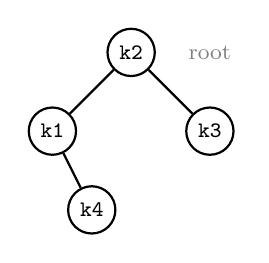
\begin{tikzpicture}

\tikzset{
    basicnode/.style={
        shape=circle,
        draw=black,
        thick,
        fill=white,
        minimum size=6mm,
        inner sep=0pt
    }
}

\node[basicnode] (m1) at (0,0) {\footnotesize\texttt{k2}};
\node[basicnode] (m2) at (-1,-1) {\footnotesize\texttt{k1}};
\node[basicnode] (m3) at (1,-1) {\footnotesize\texttt{k3}};
\node[basicnode] (m4) at (-0.5,-2) {\footnotesize\texttt{k4}};

\node[right of =m1,xshift=-0mm, smallgraytext] {root};
\draw[thick] (m1) edge (m2);
\draw[thick] (m1) edge (m3);
\draw[thick] (m2) edge (m4);
\end{tikzpicture}
\end{figure}
\end{frame}

\begin{frame}[fragile]
An \texttt{Ordict} stores \texttt{OrdictNode} objects and supports the following operations:\\~\\
\begin{itemize}

\item \highlight{\texttt{insert}} \\
\graytext{inserts/updates an object}\\[-1mm]
\begin{lstlisting}[style=mypython]
insert(key: Key, obj: Object) -> Optional[OrdictNode]
\end{lstlisting}

\item \highlight{\texttt{get}} \\
\graytext{returns an object (if it exists)}\\[-1mm]
\begin{lstlisting}[style=mypython]
get(key: Key) -> Optional[OrdictNode]
\end{lstlisting}

\item \highlight{\texttt{delete}} \\
\graytext{removes an object (if it exists)}\\[-1mm]
\begin{lstlisting}[style=mypython]
delete(key: Key) -> Optional[OrdictNode]
\end{lstlisting}

\end{itemize}
\end{frame}


\begin{frame}
\begin{center}
\Large \highlight{\texttt{Ordict}} \\[1mm]
\normalsize \color{gray} (via Balanced Binary Search Trees)
\end{center}
\end{frame}

\begin{frame}
The routing table can be stored as a binary search tree:
\begin{figure}
\centering
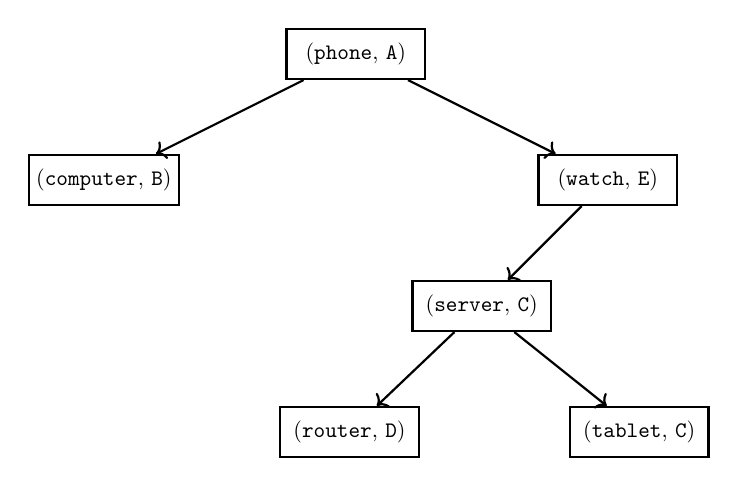
\begin{tikzpicture}[scale=0.8, transform shape]
\node (n1) at (0,0) [thick, rectangle, black, draw, minimum width=2.2cm, minimum height=8mm] {(\texttt{phone}, \labelednode{\texttt{A}}) };
\node (n2) at (-4,-2) [thick, rectangle, black, draw, minimum width=2.2cm, minimum height=8mm] {(\texttt{computer}, \labelednode{\texttt{B}})};
\node (n3) at (4,-2) [thick, rectangle, black, draw, minimum width=2.2cm, minimum height=8mm] {(\texttt{watch}, \labelednode{\texttt{E}})};
\node (n4) at (2,-4) [thick, rectangle, black, draw, minimum width=2.2cm, minimum height=8mm] {(\texttt{server}, \labelednode{\texttt{C}})};
\node (n5) at (-0.1,-6) [thick, rectangle, black, draw, minimum width=2.2cm, minimum height=8mm] {(\texttt{router}, \labelednode{\texttt{D}})};
\node (n6) at (4.5,-6) [thick, rectangle, black, draw, minimum width=2.2cm, minimum height=8mm] {(\texttt{tablet}, \labelednode{\texttt{C}})};

\draw[defaultnode, ->] (n1) -- (n2);
\draw[defaultnode, ->] (n1) -- (n3);

\draw[defaultnode, ->] (n3) -- (n4);
\draw[defaultnode, ->] (n4) -- (n5);

\draw[defaultnode, ->] (n4) -- (n6);

\end{tikzpicture}
\end{figure}
\end{frame}

\begin{frame}
\begin{thmbox}
A \highlight{\textbf{binary search tree}} is a binary tree in which each node's key is:
\begin{itemize}
\item greater than all keys in its left sub-tree, and
\item less than all keys in its right sub-tree
\end{itemize}
\begin{center}
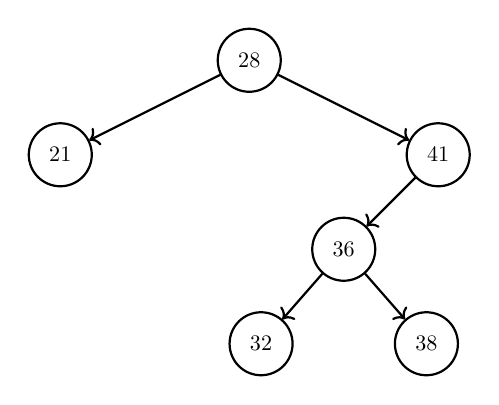
\begin{tikzpicture}[scale=0.8, transform shape]
\node[defaultnode] (n1) at (0,0)  { 28 };
\node[defaultnode] (n2) at (-3,-1.5)  { 21 };
\node[defaultnode] (n3) at (3,-1.5)  { 41 };
\node[defaultnode] (n4) at (1.5,-3)  { 36 };
\node[defaultnode] (n5) at (0.1875,-4.5)  {32};
\node[defaultnode] (n6) at (2.8125,-4.5)  {38};

\draw[defaultnode, ->] (n1) -- (n2);
\draw[defaultnode, ->] (n1) -- (n3);

\draw[defaultnode, ->] (n3) -- (n4);
\draw[defaultnode, ->] (n4) -- (n5);

\draw[defaultnode, ->] (n4) -- (n6);

\end{tikzpicture}
\end{center}
\end{thmbox}

\end{frame}

\begin{frame}[fragile]
\vspace{-7mm}
\begin{thmboxtop}
\highlight{\texttt{Ordict}} \\
\graytext{(via Balanced Binary Search Trees)}
\begin{lstlisting}[style=mypython]
class OrdictNode:
    # the key of this node
    key: Key
    
    # the object of this node
    obj: Object

    # the left child of this node
    left: Optional[OrdictNode]

    # the right child of this node
    right: Optional[OrdictNode]

    # the parent of this node
    pnt: Optional[OrdictNode]
\end{lstlisting}
\end{thmboxtop}
\end{frame}

\begin{frame}[fragile]
\begin{thmboxbot}
\begin{lstlisting}[style=mypython, firstnumber=last]
class Ordict:
# attributes
    # the root
    root: Optional[OrdictNode]
    
    # the number of nodes
    size: Integer

# functions
    ...
\end{lstlisting}
\end{thmboxbot}
\end{frame}
\begin{frame}
\begin{center}
\highlight{\textbf{insert}} \\
\footnotesize\color{gray} \texttt{insert(32, obj)}
\end{center}
\begin{center}
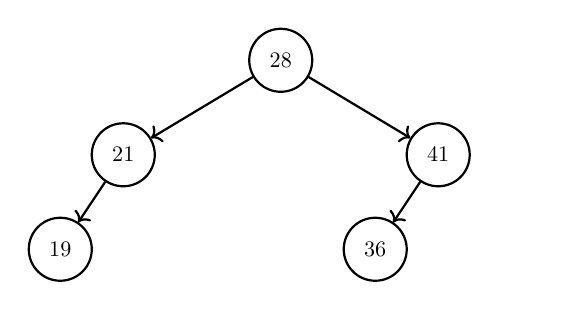
\begin{tikzpicture}[scale=0.8, transform shape, baseline=(current bounding box.north)]
\node[defaultnode] (n1) at (0,0)  { 28 };
\node[defaultnode] (n2) at (-2.5,-1.5)  { 21 };
\node[defaultnode] (n3) at (2.5,-1.5)  { 41 };
\node[defaultnode] (n4) at (1.5,-3)  { 36 };
\node[defaultnode, opacity=0] (n6) at (3.5,-3)  {v};
\node[defaultnode] (n7) at (-3.5,-3)  { 19 };

\draw[defaultnode, ->] (n1) -- (n2);
\draw[defaultnode, ->] (n1) -- (n3);

\draw[defaultnode, ->] (n3) -- (n4);
\draw[defaultnode, ->] (n2) -- (n7);

\end{tikzpicture}
\end{center}
\begin{center}
\footnotesize\color{gray} \;
\end{center}
\end{frame}

\begin{frame}
\begin{center}
\highlight{\textbf{insert}} \\
\footnotesize\color{gray} \texttt{insert(32, obj)}
\end{center}
\begin{center}
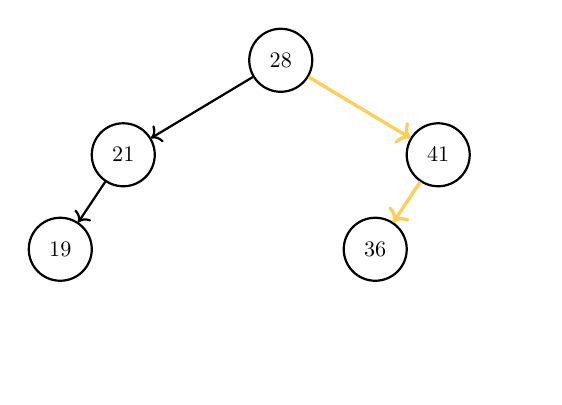
\begin{tikzpicture}[scale=0.8, transform shape, baseline=(current bounding box.north)]
\node[defaultnode] (n1) at (0,0)  { 28 };
\node[defaultnode] (n2) at (-2.5,-1.5)  { 21 };
\node[defaultnode] (n3) at (2.5,-1.5)  { 41 };
\node[defaultnode] (n4) at (1.5,-3)  { 36 };
\node[defaultnode, opacity=0] (n5) at (0.1875,-4.5)  {32};
\node[defaultnode, opacity=0] (n6) at (3.5,-3)  {v};
\node[defaultnode] (n7) at (-3.5,-3)  { 19 };

\draw[defaultnode, ->] (n1) -- (n2);
\draw[newnode, ->] (n1) -- (n3);

\draw[newnode, ->] (n3) -- (n4);
\draw[thick, ->, opacity=0] (n4) -- (n5);

\draw[defaultnode, ->] (n2) -- (n7);

\end{tikzpicture}
\end{center}
\begin{center}
\footnotesize\color{gray} find the eventual parent of the new node
\end{center}
\end{frame}

\begin{frame}
\begin{center}
\highlight{\textbf{insert}} \\
\footnotesize\color{gray} \texttt{insert(32, obj)}
\end{center}
\begin{center}
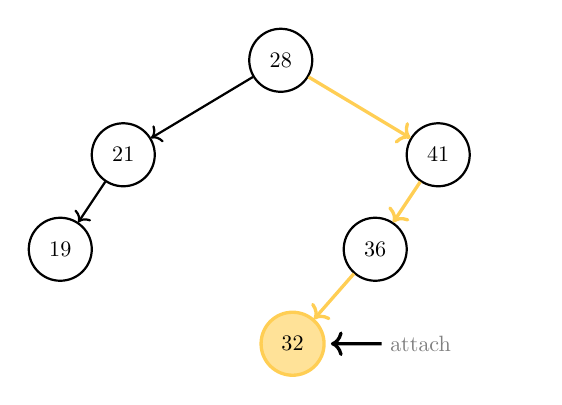
\begin{tikzpicture}[scale=0.8, transform shape, baseline=(current bounding box.north)]
\node[defaultnode] (n1) at (0,0)  { 28 };
\node[defaultnode] (n2) at (-2.5,-1.5)  { 21 };
\node[defaultnode] (n3) at (2.5,-1.5)  { 41 };
\node[defaultnode] (n4) at (1.5,-3)  { 36 };
\node[newnode] (n5) at (0.1875,-4.5) {32};
\node[defaultnode, opacity=0] (n6) at (3.5,-3)  {v};
\node[defaultnode] (n7) at (-3.5,-3)  { 19 };

\draw[defaultnode, ->] (n1) -- (n2);
\draw[newnode, ->] (n1) -- (n3);

\draw[newnode, ->] (n3) -- (n4);
\draw[newnode, ->] (n4) -- (n5);

\draw[defaultnode, ->] (n2) -- (n7);

\draw[very thick, shorten >=2pt, shorten <=2pt, <-]
(n5) edge node[right=4mm] {\color{gray} attach} ([xshift=1.5cm]n5);

\end{tikzpicture}
\end{center}
\begin{center}
\footnotesize\color{gray} attach the new node to the parent
\end{center}
\end{frame}

\begin{frame}
\begin{center}
\highlight{\textbf{insert}} \\
\footnotesize\color{gray} \texttt{insert(32, obj)}
\end{center}
\begin{center}
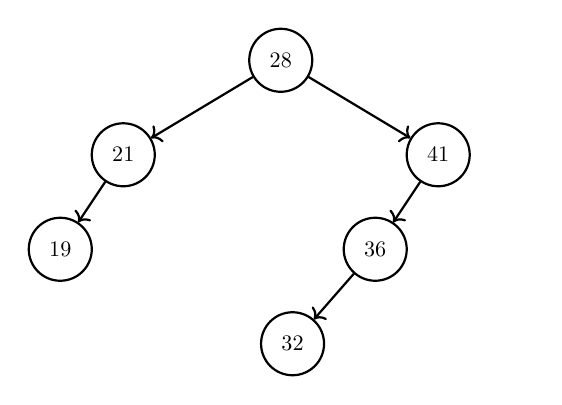
\begin{tikzpicture}[scale=0.8, transform shape, baseline=(current bounding box.north)]
\node[defaultnode] (n1) at (0,0)  { 28 };
\node[defaultnode] (n2) at (-2.5,-1.5)  { 21 };
\node[defaultnode] (n3) at (2.5,-1.5)  { 41 };
\node[defaultnode] (n4) at (1.5,-3)  { 36 };
\node[defaultnode] (n5) at (0.1875,-4.5)  {32};
\node[defaultnode, opacity=0] (n6) at (3.5,-3)  {v};
\node[defaultnode] (n7) at (-3.5,-3)  { 19 };

\draw[defaultnode, ->] (n1) -- (n2);
\draw[defaultnode, ->] (n1) -- (n3);

\draw[defaultnode, ->] (n3) -- (n4);
\draw[defaultnode, ->] (n4) -- (n5);

\draw[defaultnode, ->] (n2) -- (n7);

\end{tikzpicture}
\end{center}
\begin{center}
\footnotesize\color{gray} \;
\end{center}
\end{frame}



\begin{frame}[fragile]
\vspace{-8mm}
\begin{thmboxtop}
\begin{lstlisting}[style=mypython]
def insert(self: Ordict, key: Key, obj: Object) -> Optional[OrdictNode]:
    def _insert(self: Ordict, key: Key, curr: OrdictNode, obj: Object) -> Optional[OrdictNode]:
    if curr.key > key:
        if curr.left:
            return self._insert(curr.left, obj)
        curr.left = OrdictNode(key, obj)
        curr.left.pnt = curr
        return curr.left
        if curr.key < key:
            if curr.right:
                return self._insert(curr.right, obj)
            curr.right = OrdictNode(key, Object)
            curr.right.pnt = curr
            return curr.right
        curr.obj = obj # the key already exists
        return curr
\end{lstlisting}
\end{thmboxtop}
\end{frame}

\begin{frame}[fragile]
\begin{thmboxbot}
\begin{lstlisting}[style=mypython, firstnumber=last]
    self.size += 1
    if self.root is None:
        self.root = Ordict(key, obj)
        return self.root
    return self._insert(self.root, key, obj)
\end{lstlisting}
\end{thmboxbot}
\end{frame}

\begin{frame}[fragile]
\begin{proofbox}
\begin{lstlisting}[style=mypython]    
def get(self: Ordict, key: Key) -> Optional[OrdictNode]:
    # helper
    def _get(self: Ordict, curr: OrdictNode, key: Key) -> Optional[OrdictNode]:
        if curr is None:
            return None
        if key < curr.key:
            return self._get(curr.left, key)
        if key > curr.key:
            return self._get(curr.right, key)
        return curr
    
    if self.root:
        return self._get(self.root, key)
    return None
\end{lstlisting}
\end{proofbox}
\end{frame}

\begin{frame}[fragile]
\begin{thmbox}
\begin{lstlisting}[style=mypython]    
def delete(self: Ordict, key: Key) -> Optional[OrdictNode]:
    if self.root:
        self.size -= 1
        deleted = self._delete(self.root, key)
        return deleted
    return None
\end{lstlisting}
\end{thmbox}
\end{frame}

\begin{frame}[fragile]
\vspace{-5mm}
\begin{thmbox}
\begin{lstlisting}[style=mypython]    
def _delete(self: Ordict, curr: OrdictNode, key: Key) -> Optional[OrdictNode]:
    if curr is None:
        return None

    if key < curr.key:
        curr.left = self._delete(curr.left, key)
        if curr.left:
            curr.left.pnt = curr
        return curr

    if key > curr.key:
        curr.right = self._delete(curr.right, key)
        if curr.right:
            curr.right.pnt = curr
        return curr
        
    ...
\end{lstlisting}
\end{thmbox}
\end{frame}

\begin{frame}[fragile]
\vspace{-5mm}
\begin{thmbox}
\begin{lstlisting}[style=mypython]
    ...
    
    # no children
    if curr.left is None and curr.right is None:
        return None
    # one child
    if curr.left is None:
        curr.right.pnt = curr.pnt
        return curr.right
    if curr.right is None:
        curr.left.pnt = curr.pnt
        return curr.left
    # two children (find inorder successor)
    if curr.left.val < curr.right.val:
        succ = curr.left
    else:
        succ = curr.right
    curr.label = succ.label
    curr.obj = successor.obj
    curr.right = self._delete(curr.right, successor.key)
    if curr.right:
        curr.right.pnt = curr
    return curr
\end{lstlisting}
\end{thmbox}
\end{frame}

\begin{frame}
\begin{thmbox}
The \highlight{\textbf{balance factor}} of a node, $n$ in a tree is the difference in height between its left and right sub-trees:
\[\textsf{bf}(n) = \textsf{hgt}(\textsf{lch}(n)) - \textsf{hgt}(\textsf{rch}(n)).\]
A node in a binary search tree is \highlight{\textbf{balanced}} if $|\textsf{bf}(n)| \leq 1$.
\end{thmbox}

\begin{thmbox}
The \highlightc{myred}{\textbf{anchor}} is the first \textit{unbalanced} node on the path from the inserted node to the root. 
\end{thmbox}

\renewcommand\thefootnote{}\footnotetext{\color{gray} the balance factor can be defined the other way as well}
    
\end{frame}

\begin{frame}
\begin{center}
\highlight{\textbf{insert}} \\
\footnotesize\color{gray} \texttt{insert(32, obj)}
\end{center}
\begin{center}
\begin{tikzpicture}[scale=0.8, transform shape]
\node[defaultnode] (n1) at (0,0)  { 28 };
\node[defaultnode] (n2) at (-2.5,-1.5)  { 21 };
\node[defaultnode, fill=myred!80, draw=myred] (n3) at (2.5,-1.5)  { 41 };
\node[defaultnode] (n4) at (1.5,-3)  { 36 };
\node[newnode] (n5) at (0.1875,-4.5) {32};
\node[defaultnode] (n7) at (-3.5,-3)  { 19 };

\draw[defaultnode, ->] (n1) -- (n2);
\draw[newnode, ->] (n1) -- (n3);

\draw[newnode, ->] (n3) -- (n4);
\draw[newnode, ->] (n4) -- (n5);

\draw[defaultnode, ->] (n2) -- (n7);

\node[right = 5mm of n5, fill=lightgray!60, rounded rectangle, outer sep = 0, text width=1.2cm, align=center] {\color{gray} \faBalanceScale\; 0};


\node[left = 5mm of n4, fill=lightgray!60, rounded rectangle, outer sep = 0, text width=1.2cm, align=center] {\color{gray} \faBalanceScale\; 1};

\node[right = 5mm of n3, fill=lightgray!60, rounded rectangle, outer sep = 0, text width=1.2cm, align=center] {\color{gray}\faBalanceScale\; 2};

\node[right = 5mm of n1, fill=lightgray!60, rounded rectangle, outer sep = 0, text width=1.2cm, align=center] {\color{gray}  \faBalanceScale\; 1};
\end{tikzpicture}
\end{center}
\end{frame}

% Right Rotation

\begin{frame}
\begin{center}
    \highlight{\textbf{right rotation}} \\[2mm] \footnotesize\color{gray}
    anchor becomes unbalanced after \\
    insertion into the left sub-tree of the anchor's left child
\end{center}
\vspace{-2mm}
\begin{minipage}[t][4cm][t]{0.6\textwidth}
\centering
\begin{tikzpicture}[scale=0.8, transform shape, baseline=(current bounding box.north)]
\node (r) at (0,1.5);
\node[defaultnode] (z) at (0,0)  { \texttt{a} };
\node[defaultnode] (y) at (-1.5,-1.5)  { \texttt{c} };
\node (alpha) at (1, -1) { $\alpha$ };
\node (beta) at (-0.5, -2.5)  { $\beta$ };

\node[thick, fill=myyellow!60,
       shape=regular polygon, regular polygon sides=3,
       draw=myyellow, minimum size=14mm, inner sep=1pt]
       (new) at (-3,-3) {};

\draw[defaultnode, ->] (r) -- (z);
\draw[defaultnode, ->] (z) -- (y);
\draw[defaultnode, ->] (y) -- (new);
\draw[defaultnode, ->] (z) -- (alpha);
\draw[defaultnode, ->] (y) -- (beta);

\node[left = 4mm of new, text color = black, fill=lightgray!60, rounded rectangle, outer sep = 0, text width = 1.2cm, align=center] {\color{gray}\faRuler\;$x$};
\node[left = 5mm of y, text color = black, fill=lightgray!60, rounded rectangle, outer sep = 0, text width = 1.4cm, align=center] {\color{gray}\faRuler\;$x+1$};
\node[right = -1mm of alpha, text color = black, fill=lightgray!60, rounded rectangle, outer sep = 0, text width = 1.2cm, align=center] {\color{gray}\faRuler\;$x$};
\node[right = 1mm of beta, text color = black, fill=lightgray!60, rounded rectangle, outer sep = 0, text width = 1.4cm, align=center] {\color{gray}\faRuler\;$x$};

\end{tikzpicture}
\end{minipage}%
\begin{minipage}[t][4cm][t]{0.4\textwidth}
\centering
\begin{tikzpicture}[scale=0.8, transform shape, baseline=(current bounding box.north)]
\node (r) at (0,1.5);
\node[defaultnode] (y) at (0,0)  { \texttt{c} };
\node[defaultnode] (z) at (1.5, -1.5)  { \texttt{a} };
\node (alpha) at (2.5, -2.5)  { $\alpha$ };
\node (beta) at (0.5, -2.5)  { $\beta$ };

\node[thick, fill=myyellow!60,
shape=regular polygon, regular polygon sides=3,
draw=myyellow, minimum size=14mm, inner sep=1pt]
(new) at (-1.5,-1.5) {};

\draw[defaultnode, ->] (r) -- (y);
\draw[defaultnode, ->] (y) -- (z);
\draw[defaultnode, ->] (y) -- (new);
\draw[defaultnode, ->] (z) -- (alpha);
\draw[defaultnode, ->] (z) -- (beta);
\end{tikzpicture}
\end{minipage}
\begin{center}
\footnotesize\color{gray}
(heights are before insertion)
\end{center}
\end{frame}

\begin{frame}[fragile]
\begin{proofbox}
\begin{lstlisting}[style=mypython]
def rotate_right(self: Ordict, p: OrdictNode) -> OrdictNode:
    a = p.left
    if not a:
        return p 

    p.left = a.right
    a.right = p
    return a
\end{lstlisting}    
\end{proofbox}

\end{frame}

\begin{frame}
\begin{center}
\highlight{\textbf{left rotation}} \\[2mm] \footnotesize\color{gray}
anchor becomes unbalanced after \\
inserting into the right sub-tree of the anchor's right child
\end{center}
\vspace{-2mm}
\begin{minipage}[t][4cm][t]{0.6\textwidth}
\centering
\begin{tikzpicture}[scale=0.8, transform shape, xscale=-1, baseline=(current bounding box.north)]
\node (r) at (0,1.5);
\node[defaultnode](z) at (0,0)  { \texttt{a} };
\node[defaultnode,   xscale=-1] (y) at (-1.5,-1.5)  { \texttt{c} };
\node[ xscale=-1] (alpha) at (1, -1) [circle, minimum width=11mm] { $\alpha$ };
\node[ xscale=-1] (beta) at (-0.5, -2.5)  { $\beta$ };

\node[thick, fill=myyellow!60,
shape=regular polygon, regular polygon sides=3,
draw=myyellow, minimum size=14mm, inner sep=1pt]
(new) at (-3,-3) {};

\draw[defaultnode, ->] (r) -- (z);
\draw[defaultnode, ->] (z) -- (y);
\draw[defaultnode, ->] (y) -- (new);
\draw[defaultnode, ->] (z) -- (alpha);
\draw[defaultnode, ->] (y) -- (beta);


\node[xscale=-1, right = -12mm of new, text color = black, fill=lightgray!60, rounded rectangle, outer sep = 0, text width = 1.2cm, align=center] {\color{gray}\faRuler\;$x$};
\node[xscale=-1, right = -5mm of y, text color = black, fill=lightgray!60, rounded rectangle, outer sep = 0, text width = 1.4cm, align=center] {\color{gray}\faRuler\;$x+1$};
\node[xscale=-1, left = 1mm of alpha, text color = black, fill=lightgray!60, rounded rectangle, outer sep = 0, text width = 1.2cm, align=center] {\color{gray}\faRuler\;$x$};
\node[xscale=-1, left = -1mm of beta, text color = black, fill=lightgray!60, rounded rectangle, outer sep = 0, text width = 1.4cm, align=center] {\color{gray}\faRuler\;$x$};

\end{tikzpicture}
\end{minipage}%
\begin{minipage}[t][4cm][t]{0.4\textwidth}
\centering
\begin{tikzpicture}[scale=0.8, transform shape, xscale=-1, baseline=(current bounding box.north)]
\node (r) at (0,1.5);
\node[defaultnode, xscale=-1](y) at (0,0) { \texttt{c} };
\node[defaultnode, xscale=-1](z) at (1.5, -1.5)  { \texttt{a} };
\node[xscale=-1] (alpha) at (2.5, -2.5) { $\alpha$ };
\node[xscale=-1] (beta) at (0.5, -2.5) { $\beta$ };

\node[thick, fill=myyellow!60,
shape=regular polygon, regular polygon sides=3,
draw=myyellow, minimum size=14mm, inner sep=1pt]
(new) at (-1.5,-1.5) {};

\draw[defaultnode, ->] (r) -- (y);
\draw[defaultnode, ->] (y) -- (z);
\draw[defaultnode, ->] (y) -- (new);
\draw[defaultnode, ->] (z) -- (alpha);
\draw[defaultnode, ->] (z) -- (beta);
\end{tikzpicture}
\end{minipage}
\begin{center}
\footnotesize\color{gray}
(heights are before insertion)
\end{center}
\end{frame}


\begin{frame}[fragile]
\begin{proofbox}
\begin{lstlisting}[style=mypython]
def rotate_left(self: Ordict, p: OrdictNode) -> OrdictNode:
    a = p.right
    if not a:
        return p 

    p.right = a.left
    a.left = p
    return a
\end{lstlisting}    
\end{proofbox}

\end{frame}

\begin{frame}
\vspace{-5mm}
\begin{center}
\highlight{\textbf{left-right rotation}} \\[2mm] \footnotesize\color{gray}
anchor becomes unbalanced after \\
insertion into the right sub-tree of the anchor's left child
\end{center}
\vspace{-5mm}
\begin{minipage}[t][5cm][t]{0.6\textwidth}
\centering
\begin{tikzpicture}[scale=0.8, transform shape, xscale=-1, baseline=(current bounding box.north)]
\node (r) at (0,1.5);
\node[defaultnode, xscale=-1](p) at (0,0)  {\texttt{a}};
\node[defaultnode, xscale=-1](a) at (1.5,-1.5)  {\texttt{c}};
\node[defaultnode, xscale=-1](c) at (0,-3)  {\texttt{g}};
\node[xscale=-1] (alpha) at (-2, -1.5) {$\alpha$};
\node[newnode, xscale=-1] (beta) at (-1, -4) {$\beta$};
\node[xscale=-1] (delta) at (2.5, -2.5) {$\delta$};

\node[thick, fill=myyellow!60,
       shape=regular polygon, regular polygon sides=3,
       draw=myyellow, minimum size=14mm, inner sep=1pt]
       (new) at (1,-4) {};

\draw[defaultnode, ->] (r) -- (p);
\draw[defaultnode, ->] (p) -- (a);
\draw[defaultnode, ->] (p) -- (alpha);
\draw[defaultnode, ->] (a) -- (c);
\draw[defaultnode, ->] (a) -- (delta);
\draw[defaultnode, ->] (c) -- (beta);
\draw[defaultnode, ->] (c) -- (new);

\node[xscale=-1, right = -15mm of y, text color = black, fill=lightgray!60, rounded rectangle, outer sep = 0, text width = 1.4cm, align=center] {\color{gray}\faRuler\;$x+2$};
\node[xscale=-1, right = 1mm of alpha, text color = black, fill=lightgray!60, rounded rectangle, outer sep = 0, text width = 1.2cm, align=center] {\color{gray}\faRuler\;$x$};
\node[xscale=-1, left = -4mm of a, text color = black, fill=lightgray!60, rounded rectangle, outer sep = 0, text width = 1.4cm, align=center] {\color{gray}\faRuler\;$x+1$};
\node[xscale=-1, right = -4mm of beta, text color = black, fill=lightgray!60, rounded rectangle, outer sep = 0, text width = 1.6cm, align=center] {\color{gray}\faRuler\;$x-1$};
\node[xscale=-1, left = -12mm of new, text color = black, fill=lightgray!60, rounded rectangle, outer sep = 0, text width = 1.6cm, align=center] {\color{gray}\faRuler\;$x-1$};
\node[xscale=-1, right = -4mm of c, text color = black, fill=lightgray!60, rounded rectangle, outer sep = 0, text width = 1.4cm, align=center] {\color{gray}\faRuler\;$x$};
\node[xscale=-1, left = 0mm of delta, text color = black, fill=lightgray!60, rounded rectangle, outer sep = 0, text width = 1.4cm, align=center] {\color{gray}\faRuler\;$x$};

\end{tikzpicture}
\end{minipage}%
\begin{minipage}[t][5cm][t]{0.4\textwidth}
\centering
\begin{tikzpicture}[scale=0.8, transform shape, xscale=-1, baseline=(current bounding box.north)]
\node (r) at (0,1.5);
\node[defaultnode, xscale=-1](c) at (0,0)  {\texttt{g}};
\node[defaultnode, xscale=-1](p) at (-1.5,-1.5)  {\texttt{a}};
\node[defaultnode, xscale=-1](a) at (1.5,-1.5)  {\texttt{c}};
\node[xscale=-1] (alpha) at (-2.5, -2.5) {$\alpha$};
\node[newnode, xscale=-1] (beta) at (-0.6, -3) {$\beta$};
\node[xscale=-1] (delta) at (2.5, -2.5) {$\delta$};

\node[thick, fill=myyellow!60,
       shape=regular polygon, regular polygon sides=3,
       draw=myyellow, minimum size=14mm, inner sep=1pt]
       (new) at (0.6,-3) {};

\draw[defaultnode, ->] (r) -- (c);
\draw[defaultnode, ->] (c) -- (p);
\draw[defaultnode, ->] (c) -- (a);
\draw[defaultnode, ->] (p) -- (alpha);
\draw[defaultnode, ->] (p) -- (beta);
\draw[defaultnode, ->] (a) -- (new);
\draw[defaultnode, ->] (a) -- (delta);
\end{tikzpicture}
\end{minipage}
\begin{center}
\footnotesize\color{gray}
(heights are before insertion)
\end{center}
\renewcommand\thefootnote{}\footnotetext{\color{gray} insertion can be done at $\beta$ instead of at \raisebox{1.5mm}{\rotatebox{180}{\triangleicon}}}
\end{frame}

\begin{frame}[fragile]
\begin{proofbox}
\begin{lstlisting}[style=mypython]
def rotate_left_right(self, p):
    if not p.left:
        return p
    p.left = self.rotate_left(p.left)
    return self.rotate_right(p)
\end{lstlisting}    
\end{proofbox}
\end{frame}


\begin{frame}
\begin{center}
    \highlight{\textbf{right-left rotation}} \\[2mm] \footnotesize\color{gray}
    after insertion into the left sub-tree of the anchor's right child \\
    making the anchor unbalanced
\end{center}
\vspace{-5mm}
\begin{minipage}[t][5mm][t]{0.6\textwidth}
\centering
\begin{tikzpicture}[scale=0.8, transform shape, baseline=(current bounding box.north)]
\node (r) at (0,1.5);
\node[defaultnode,  xscale=1] (p) at (0,0)  {\texttt{a}};
\node[defaultnode,  xscale=1] (a) at (1.5,-1.5)  {\texttt{c}};
\node[defaultnode,  xscale=1] (c) at (0,-3)  {\texttt{g}};
\node (alpha) at (-2, -1.5) [circle, minimum width=11mm, xscale=1] {$\alpha$};
\node[newnode] (beta) at (-1, -4) {$\beta$};
\node (delta) at (2.5, -2.5) [circle, minimum width=11mm, xscale=1] {$\delta$};

\node[thick, fill=myyellow!60,
       shape=regular polygon, regular polygon sides=3,
       draw=myyellow, minimum size=14mm, inner sep=1pt]
       (new) at (1,-4) {};

\draw[defaultnode, ->] (r) -- (p);
\draw[defaultnode, ->] (p) -- (a);
\draw[defaultnode, ->] (p) -- (alpha);
\draw[defaultnode, ->] (a) -- (c);
\draw[defaultnode, ->] (a) -- (delta);
\draw[defaultnode, ->] (c) -- (beta);
\draw[defaultnode, ->] (c) -- (new);

\node[xscale=1, left = 15mm of y, text color = black, fill=lightgray!60, rounded rectangle, outer sep = 0, text width = 1.4cm, align=center] {\color{gray}\faRuler\;$x+2$};
\node[xscale=1, left = 0mm of alpha, text color = black, fill=lightgray!60, rounded rectangle, outer sep = 0, text width = 1.2cm, align=center] {\color{gray}\faRuler\;$x$};
\node[xscale=1, right = 4mm of a, text color = black, fill=lightgray!60, rounded rectangle, outer sep = 0, text width = 1.4cm, align=center] {\color{gray}\faRuler\;$x+1$};
\node[xscale=1, left = 4mm of beta, text color = black, fill=lightgray!60, rounded rectangle, outer sep = 0, text width = 1.6cm, align=center] {\color{gray}\faRuler\;$x-1$};
\node[xscale=1, right = 6mm of new, text color = black, fill=lightgray!60, rounded rectangle, outer sep = 0, text width = 1.6cm, align=center] {\color{gray}\faRuler\;$x-1$};
\node[xscale=1, left = 4mm of c, text color = black, fill=lightgray!60, rounded rectangle, outer sep = 0, text width = 1.4cm, align=center] {\color{gray}\faRuler\;$x$};
\node[xscale=1, right = 0mm of delta, text color = black, fill=lightgray!60, rounded rectangle, outer sep = 0, text width = 1.4cm, align=center] {\color{gray}\faRuler\;$x$};

\end{tikzpicture}
\end{minipage}%
\begin{minipage}[t][5cm][t]{0.4\textwidth}
\centering
\begin{tikzpicture}[scale=0.8, transform shape, baseline=(current bounding box.north)]
\node (r) at (0,1.5);
\node[defaultnode, xscale=1] (c) at (0,0)  {\texttt{g}};
\node[defaultnode, xscale=1] (p) at (-1.5,-1.5)  {\texttt{a}};
\node[defaultnode, xscale=1] (a) at (1.5,-1.5)  {\texttt{c}};
\node (alpha) at (-2.5, -2.5) [circle, minimum width=11mm, xscale=1] {$\alpha$};
\node[newnode] (beta) at (-0.6, -3) {$\beta$};
\node (delta) at (2.5, -2.5) [circle, minimum 
+width=11mm, xscale=1] {$\delta$};

\node[thick, fill=myyellow!60,
       shape=regular polygon, regular polygon sides=3,
       draw=myyellow, minimum size=14mm, inner sep=1pt]
       (new) at (0.6,-3) {};

\draw[defaultnode, ->] (r) -- (c);
\draw[defaultnode, ->] (c) -- (p);
\draw[defaultnode, ->] (c) -- (a);
\draw[defaultnode, ->] (p) -- (alpha);
\draw[defaultnode, ->] (p) -- (beta);
\draw[defaultnode, ->] (a) -- (new);
\draw[defaultnode, ->] (a) -- (delta);
\end{tikzpicture}
\end{minipage}

\begin{center}
\footnotesize\color{gray}
(heights are before insertion)
\end{center}
\renewcommand\thefootnote{}\footnotetext{\color{gray} insertion can be done at $\beta$ instead of at \raisebox{1.5mm}{\rotatebox{180}{\triangleicon}}}
\end{frame}

\begin{frame}[fragile]
\begin{proofbox}
\begin{lstlisting}[style=mypython]
def rotate_right_left(self: Ordict, p: OrdictNode) -> OrdictNode:
    if not p.right:
        return p
    p.right = self.rotate_right(p.right)
    return self.rotate_left(p)
\end{lstlisting}    
\end{proofbox}
\end{frame}

\begin{frame}[fragile]
\vspace{-5mm}
\begin{thmbox}
\begin{lstlisting}[style=mypython]
def _insert(self: Ordict, curr: OrdictNode, obj: Object) -> Optional[OrdictNode]:
    ...
    balance = self.get_balance(curr)

    # left-left
    if balance > 1 and key < curr.left.key:
        return self.rotate_right(curr)
    # right-right
    if balance < -1 and key > curr.right.key:
        return self.rotate_left(curr)
    # left-right
    if balance > 1 and key > curr.left.key:
        return self.rotate_left_right(curr)
    # right-left
    if balance < -1 and key < curr.right.key:
        return self.rotate_right_left(curr)
    return curr
\end{lstlisting}
\end{thmbox}
\end{frame}

\begin{frame}
\begin{center}
\highlight{\textbf{insert}} \\
\footnotesize\color{gray} \texttt{insert(38, obj)}
\end{center}
\begin{center}
\begin{tikzpicture}[scale=0.8, transform shape]
\node[defaultnode] (n1) at (0,0)  { 28 };
\node[defaultnode] (n2) at (-2.5,-1.5)  { 21 };
\node[defaultnode, fill=myred!80, draw=myred] (n3) at (2.5,-1.5)  { 41 };
\node[defaultnode] (n4) at (1.5,-3)  { 36 };
\node[newnode] (n5) at (0.1875,-4.5) {32};
\node[defaultnode] (n7) at (-3.5,-3)  { 19 };

\draw[defaultnode, ->] (n1) -- (n2);
\draw[newnode, ->] (n1) -- (n3);

\draw[newnode, ->] (n3) -- (n4);
\draw[newnode, ->] (n4) -- (n5);

\draw[defaultnode, ->] (n2) -- (n7);

\node[right = 5mm of n5, fill=lightgray!60, rounded rectangle, outer sep = 0, text width=1.2cm, align=center] {\color{gray} \faBalanceScale\; 0};


\node[left = 5mm of n4, fill=lightgray!60, rounded rectangle, outer sep = 0, text width=1.2cm, align=center] {\color{gray} \faBalanceScale\; 1};

\node[right = 5mm of n3, fill=lightgray!60, rounded rectangle, outer sep = 0, text width=1.2cm, align=center] {\color{gray}\faBalanceScale\; 2};

\node[right = 5mm of n1, fill=lightgray!60, rounded rectangle, outer sep = 0, text width=1.2cm, align=center] {\color{gray}  \faBalanceScale\; 1};
\end{tikzpicture}
\end{center}
\begin{center}
    \footnotesize\color{gray} (before rotation)
\end{center}
\end{frame}

\begin{frame}
\begin{center}
\highlight{\textbf{insert}} \\
\footnotesize\color{gray} \texttt{insert(38, obj)}
\end{center}
\begin{center}
\begin{tikzpicture}[scale=0.8, transform shape]
\draw[opacity=0] (-7,-5) rectangle (7,1);
\node[defaultnode] (n1) at (0,0)  { 28 };
\node[defaultnode] (n2) at (-2.5,-1.5)  { 21 };
\node[defaultnode] (n3) at (2.5,-1.5)  { 36 };
\node[defaultnode] (n4) at (1.5,-3)  { 32 };
\node[defaultnode] (n6) at (3.5,-3)  {41};
\node[defaultnode] (n7) at (-3.5,-3)  { 19 };

\draw[defaultnode, ->] (n1) -- (n2);
\draw[defaultnode, ->] (n1) -- (n3);

\draw[defaultnode, ->] (n3) -- (n4);

\draw[defaultnode, ->] (n3) -- (n6);
\draw[defaultnode, ->] (n2) -- (n7);

\node[right = 5mm of n6, fill=lightgray!60, rounded rectangle, outer sep = 0, text width=1.2cm, align=center] {\color{gray} \faBalanceScale\; 0};


\node[left = 5mm of n4, fill=lightgray!60, rounded rectangle, outer sep = 0, text width=1.2cm, align=center] { \color{gray}\faBalanceScale\; 0};

\node[right = 5mm of n3, fill=lightgray!60, rounded rectangle, outer sep = 0, text width=1.2cm, align=center] {\color{gray}\faBalanceScale\; 0};

\node[right = 5mm of n1, fill=lightgray!60, rounded rectangle, outer sep = 0, text width=1.2cm, align=center] { \color{gray}\faBalanceScale\; 0};

\node[left = 5mm of n7, fill=lightgray!60, rounded rectangle, outer sep = 0, text width=1.2cm, align=center] { \color{gray}\faBalanceScale\; 0};

\node[left = 5mm of n2, fill=lightgray!60, rounded rectangle, outer sep = 0, text width=1.2cm, align=center] { \color{gray}\faBalanceScale\; 1};
\end{tikzpicture}
\end{center}
\begin{center}
    \footnotesize\color{gray}(after rotation)
\end{center}
\end{frame}

\begin{frame}
\begin{center}
\Large \highlight{\textbf{appendix}} \\[1mm]
\normalsize\color{gray} (proofs)
    
\end{center}    
\end{frame}

\begin{frame}
\begin{table}
\begin{tabular}{@{} r | l @{} }
\highlight{\textbf{Property}} & \\[1mm]\hline
\multirow{1}{*}{Time Complexity} & \\
\color{gray}\footnotesize\texttt{insert} & \color{gray}\footnotesize $O(\log(N))$\\[1mm]
\color{gray}\footnotesize\texttt{get} & \color{gray}\footnotesize $O(\log(N))$ \\[1mm]
\color{gray}\footnotesize\texttt{delete} & \color{gray}\footnotesize $O(\log(N))$\\[1mm]
Space Complexity & $O(N)$
\end{tabular}
\end{table}
\begin{center}
\footnotesize\color{gray} properties of the \texttt{Ordict} data-structure (via Balanced Binary Search Trees)
\end{center}
\renewcommand\thefootnote{}\footnotetext{\color{gray} Assumptions: $N = $ \texttt{Ordict.count}}
\end{frame}

\begin{frame}
\vspace{-5mm}
\begin{thmbox}
The time complexity of \texttt{insert} for \texttt{Ordict} (via Balanced Binary Search Trees) is $O(\log N)$, where $N=\texttt{Ordict.size}$.
\end{thmbox}
\begin{thmboxtop}
\normalsize\color{black}
\highlightc{lightgray}{\textbf{finding the new node's parent}}: \hfill $O(\log N)$
\\[1mm]
\graytext{Since the tree is balanced, its height is at most $\log(N)$.}
\begin{itemize}
\footnotesize\color{gray}
\item the \emph{worst-case} height for balanced tree of given size (\# of nodes) occurs when the tree is as small as possible
\item this happens when given a node with a height of $x$, one child has a height of $x-1$ and the other has a height of $x-2$ (if they both had a height of $x-1$, this would result in a larger tree)
\item thus the size of the smallest balanced tree with height $x$, denoted $N(x)$, must satisfy the following recurrence:
\[N(x)=1+N(x-1)+N(x-2),\]
where $N(0) = 0$ and $N(1) = 1$
\end{itemize}
\end{thmboxtop}
\end{frame}

\begin{frame}
\begin{thmboxside}
\begin{itemize}
\footnotesize\color{gray}
\item it follows that $N(x) \geq 2N(x-2)$
\item solving the recurrence, we see that
\[N(x) \geq 2^{x/2} \;\; \forall x \geq 0\]
\item re-arranging tell us that
\[x \leq \log_2(N(x))\]
\end{itemize}
\graytext{
Following the search tree property, we traverse down from the root, visiting at most $O(\log N)$ nodes to find the parent of the new node.}
\end{thmboxside}
\end{frame}

\begin{frame}
\begin{thmboxbot}
\highlightc{lightgray}{\textbf{inserting the new node}}: \hfill $O(1)$
\\[1mm]
\graytext{We create and attach the new node to its parent, which takes $O(1)$ time.} \\[2mm]
\highlightc{lightgray}{\textbf{finding the anchor}}: \hfill $O(\log N)$ \\[1mm]
\graytext{The path from the new node back to the root contains at most $\ceil{\log{(N)+1}}$ nodes. We traverse this path, updating the height / balance factor at each node until the first unbalanced node is found (the anchor), or we reach the root.}
\\[2mm]
\highlightc{lightgray}{\textbf{restoring balance}}: \hfill $O(1)$
\\[1mm]
\graytext{If an anchor exists, we perform a rotation, which takes $O(1)$ time.}
\end{thmboxbot}    
\end{frame}

\begin{frame}
\vspace{-5mm}
\begin{thmbox}
The time complexity of \texttt{get} for \texttt{Ordict} (via Balanced Binary Search Trees) is $O(\log N)$, where $N=\texttt{Ordict.size}$.
\end{thmbox}
\begin{proofbox}
\normalsize\color{black}
\highlightc{lightgray}{\textbf{finding the node}}: \hfill $O(\log N)$ \\[1mm]
\footnotesize\color{gray}
Since the tree is balanced, its height is at most $\log(N)$. Following the search tree property, we traverse down from the root, visiting at most $O(\log N)$ nodes to find the target node.
\end{proofbox}
\end{frame}

\end{document}
